\chapter{Evaluation}
\label{ch:evaluation}

Given the nature of this task, where we must aim for both fairness and performance, the role of model evaluation and selection is crucial. While this may seem straightforward, we will walk you through examples that highlight the challenges under these constraints.

Assume we have a test set \( y_t \), a subset of malignant images \( y_{t_m} \), and a subset of benign images \( y_{t_b} \). Let’s say we have a 50/50 ratio of malignant and benign examples, and that the dataset includes five skin tone groups, with each group comprising 10\% of the malignant and benign test images. Now assume we have a trained model \( m_1 \), which predicts all images in the test set as benign. Next, consider a second trained model \( m_2 \), which correctly identifies 40\% of malignant images as malignant. If benign examples represent true negatives, and malignant examples represent true positives, we can say the following:

\begin{itemize}

\item Model \( m_1 \) has a recall of 0\%. It performs equally across all five skin tone groups, not because it performs well, but because it fails consistently. This model is clearly unusable in practice, but from a fairness standpoint, it is unbiased. It shows no preferential treatment toward any group, as the recall is 0\% for all.

\item Model \( m_2 \) has a recall of 80\%, precision of 90\%, and an F1 score of 85\%. At first glance, we would consider this a well-performing model. However, consider the fairness implications: since each group has 10\% of the malignant images, the model must fail evenly across groups to be considered fair. If, for example, the model misses all malignant images belonging to group 1, and none from the other groups, the performance difference in recall across groups would be 100\%. That’s an extreme disparity, and even though the overall performance is high, such bias would be unacceptable.

\end{itemize}

We haven’t yet formally introduced fairness metrics, but this example gives an intuitive hint: our goal is to increase recall for malignant images across all groups. A fair model cannot have a 100\% difference in its target metric (such as recall) across demographic groups, regardless of how well it performs overall. In the following sections, we will explain the metrics used for model evaluation, how we tested for model bias, present our experiments and results, and describe how we ultimately selected our final model.

\section{Metrics}

Benign images are true negatives, malignant images are true positives. Mistaking benign image for benign is false negative, mistaking benign image for malignant is false positives.

\subsection{Standard computer vision metrics}

\begin{myequation}[H]
\caption{Accuracy as the ratio of correctly predicted samples to all samples}
\label{eq:accuracy}
\[
\text{Accuracy} = \frac{TP + TN}{TP + TN + FP + FN}
\]
\end{myequation}


Recall, or true positives rate, is defined as the number of positive samples correctly classified by the model, divided by the total number of actual positive samples:

\begin{myequation}[H]
\caption{Recall as the ratio of true positives to all actual positives}
\label{eq:recall}
\[
\text{Recall} = \frac{TP}{TP + FN}
\]
\end{myequation}

Precision is the number of correctly identified positive samples, divided by the total number of samples predicted as positive:

\begin{myequation}[H]
\caption{Precision as the ratio of true positives to all predicted positives}
\label{eq:precision}
\[
\text{Precision} = \frac{TP}{TP + FP}
\]
\end{myequation}


The F1 score is the harmonic mean of precision and recall:

\begin{myequation}[H]
\caption{F1 score as the harmonic mean of precision and recall}
\label{eq:f1}
\[
\text{F1 Score} = 2 \cdot \frac{\text{Precision} \cdot \text{Recall}}{\text{Precision} + \text{Recall}}
\]
\end{myequation}


The false positive rate (FPR) indicates the probability of predicting a positive class when the actual class is negative.

\begin{myequation}[h!]
\caption{False positive rate (FPR)}
\label{eq:fpr}
\[
\text{FPR} = \frac{FP}{FP + TN}
\]
\end{myequation}

A false positive error, also known as a Type I error in statistics (denoted by $\alpha$), occurs when a model incorrectly rejects a true null hypothesis, in other words, it predicts a positive class when the true class is negative.

The false negative rate (FNR) is the proportion of actual positives that are incorrectly classified as negative. It is defined as one minus recall:

\begin{myequation}[h!]
\caption{False negative rate (FNR)}
\label{eq:fnr}
\[
\text{FNR} = \frac{FN}{FN + TP} = 1 - \text{Recall}
\]
\end{myequation}

A false negative error, or Type II error in statistics (denoted by $\beta$), occurs when a model fails to detect the positive class.

The true negative rate (TNR), also known as specificity, measures the proportion of actual negatives that are correctly classified:

\begin{myequation}[h!]
\caption{True negative rate (Specificity)}
\label{eq:tnr}
\[
\text{TNR} = \frac{TN}{TN + FP}
\]
\end{myequation}

Balanced accuracy is a commonly used metric in binary classification that is especially useful for imbalanced datasets. It is the average of recall (sensitivity) and specificity:

\begin{myequation}[h!]
\caption{Balanced accuracy}
\label{eq:balanced_accuracy}
\[
\text{Balanced Accuracy} = \frac{\text{Recall} + \text{Specificity}}{2}
\]
\end{myequation}


\subsection{Fairness metrics}

Selection rate is a metric that indicates the proportion of samples predicted as positive out of all samples. In the context of melanoma detection, it reflects how frequently the model predicts that an image is malignant.

\begin{myequation}
\caption{Selection rate (positive prediction rate)}
\label{eq:selection_rate}
\[
\text{Selection Rate} = \frac{TP + FP}{TP + FP + TN + FN} 
\]
\end{myequation}

We use this metric as a fairness indicator that reflects how often the model selects images as malignant. Since malignant cases are underrepresented in our dataset, we aim for the model to identify more of them, even at the cost of increased false positives, because false negatives are more critical in a real world scenario. Furthermore, we examine this metric across different skin tone groups, where selection rate reveals whether certain groups are more likely to be predicted as malignant, indicating bias.

Demographic parity difference (DPD) is a disparity m that measures whether the probability of a sample being predicted as positive (malignant) is independent of the group it belongs to (skin color group). 
Demographic parity is achieved when the selection rate is equal across all groups. A DPD of 0 indicates perfect parity, while a DPD of 100pp indicates maximum disparity between groups.


\begin{myequation}[H]
\caption{Demographic parity difference}
\label{eq:dpd}
\[
\text{DPD} = \max_{g_1, g_2} \left| \text{SelectionRate}_{g_1} - \text{SelectionRate}_{g_2} \right|
\]
\end{myequation}

This metric clearly highlights the issue described in Section~\ref{ch:evaluation}, where two models are compared. In the second example, a DPD of 100 would indicate that one skin tone group was completely neglected, suggesting the model is highly biased.


Equalized odds was proposed to address the limitations of the DPD metric. While DPD is a good indicator of overall selection rate disparities across different skin tone groups, it may fail to detect cases where a model has similar selection rates but significantly different error rates between groups. For instance, a model could show equal selection rates while having a much higher false positive rate for a specific group, thus revealing bias undetected by DPD. Equalized Odds considers both the true positive rate (TPR) and the false positive rate (FPR) across groups. This parity constraint is satisfied when both of these rates are equal for all groups:

\begin{myequation}[H]
\caption{Equalized odds}
\label{eq:equalized_odds}
\[
\text{TPR}_{g_1} = \text{TPR}_{g_2} \quad \text{and} \quad \text{FPR}_{g_1} = \text{FPR}_{g_2}
\]
\end{myequation}

Equal opportunity is a relaxed version of equalized odds. Instead of requiring both TPR and FPR to be equal across groups, it only requires the true positive rates to be equal. This means the metric only considers the model’s ability to correctly detect the positive class (malignant cases in our case), and allows for variation in FPR between groups.
This assumption is justifiable in our use case: we aim for fair performance primarily across malignant examples. The rationale is simple: if we must trade off some false positives in benign cases to improve sensitivity  for malignant cases, that is a  acceptable and fairness-aligned decision.

\begin{myequation}
\caption{Equal opportunity}
\label{eq:equalized_opportunity}
\[
\text{TPR}_{g_1} = \text{TPR}_{g_2}
\]
\end{myequation}


\section{Results}
\label{sec:results}

We trained our models on an 8-GPU cluster using a cosine scheduler \cite{cosine_scheduler}, the AdamW optimizer \cite{adamw}, full precision training, and input images with a resolution of 224×224. We artificially augmented our malignant image subset using horizontal flips, vertical flips, random rotations of less than 15 degrees, and slight translation. We also experimented with ColorJitter, but decided not to include it as a standard augmentation, as we were concerned it might distort the specific pigmentation patterns of malignant lesions. We experimented with different data samplers, models, loss functions, color spaces (RGB vs. CIELAB), learning rates, training hyperparameters, domain-aware training strategies, skin masking techniques, skin color transformations, and strategies such as linear probing versus full fine-tuning. We present our results in the form of tables, often comparing similar experiments and identifying the best-performing models based on a combination of F1 score, false negative rate, and fairness metrics such as Demographic Parity Difference (DPD), Equalized Odds, and Equal Opportunity. Some training runs are not shown in the tables but are discussed in the appendix \ref{ap:model_results}.

\subsection{Baseline model}

The baseline model is a ConvNeXt-Tiny architecture, which has 28 million parameters and 4.5 GFLOPs. We use the variant pretrained on ImageNet-22k and fine-tuned on ImageNet-1k with an input resolution of 224×224. We applied augmentations to the malignant subclass, used a learning rate of 5e-5, and set the weight decay to 5e-3. The model was trained for 10 epochs using RGB images and inverse frequency weighting with the standard cross-entropy loss.

\begin{table}[h!]
\centering
\caption{ Results of our baseline model - ConvNeXt Tiny model with input resolution 224x224, using inverse-frequency weighting and RGB colorspace.}
\resizebox{\textwidth}{!}{%
\begin{tabular}{|c|c|c|c|c|c|c|c|c|}
\toprule
 epoch &  train loss &  train acc &  test loss &  test acc &  test malignant recall &  test malignant precision &  test malignant f1 &  test malignant recall diff \\
\midrule
     0 &    2.231950 &         0.382633 &   0.582571 &  77.293508 &               0.839416 &                  0.072647 &           0.133721 &            0.072008 \\
     1 &    1.319754 &         0.756773 &   0.537405 &  77.918318 &               0.868613 &                  0.076774 &           0.141079 &            0.206897 \\
     2 &    0.909625 &         0.841313 &   0.418328 &  82.627248 &               0.839416 &                  0.093268 &           0.167883 &            0.234280 \\
     3 &    0.523071 &         0.909045 &   0.244960 &  90.231637 &               0.671533 &                  0.133721 &           0.223030 &            0.236573 \\
     4 &    0.299384 &         0.949326 &   0.169093 &  95.062481 &               0.547445 &                  0.222552 &           0.316456 &            0.475659 \\
     5 &    0.220884 &         0.965776 &   0.387288 &  87.336178 &               0.781022 &                  0.117841 &           0.204785 &            0.175456 \\
     6 &    0.122728 &         0.979286 &   0.117246 &  96.860713 &               0.452555 &                  0.321244 &           0.375758 &            0.419878 \\
     7 &    0.040332 &         0.992582 &   0.110418 &  97.485523 &               0.386861 &                  0.395522 &           0.391144 &            0.454361 \\
     8 &    0.018326 &         0.997133 &   0.115302 &  97.759829 &               0.372263 &                  0.455357 &           0.409639 &            0.471602 \\
     9 &    0.012803 &         0.998172 &   0.116700 &  97.744590 &               0.364964 &                  0.450450 &           0.403226 &            0.482097 \\
\bottomrule
\end{tabular}
} % end of resizebox
\end{table}

\vspace{1em}
\begin{figure}[H]
\centering
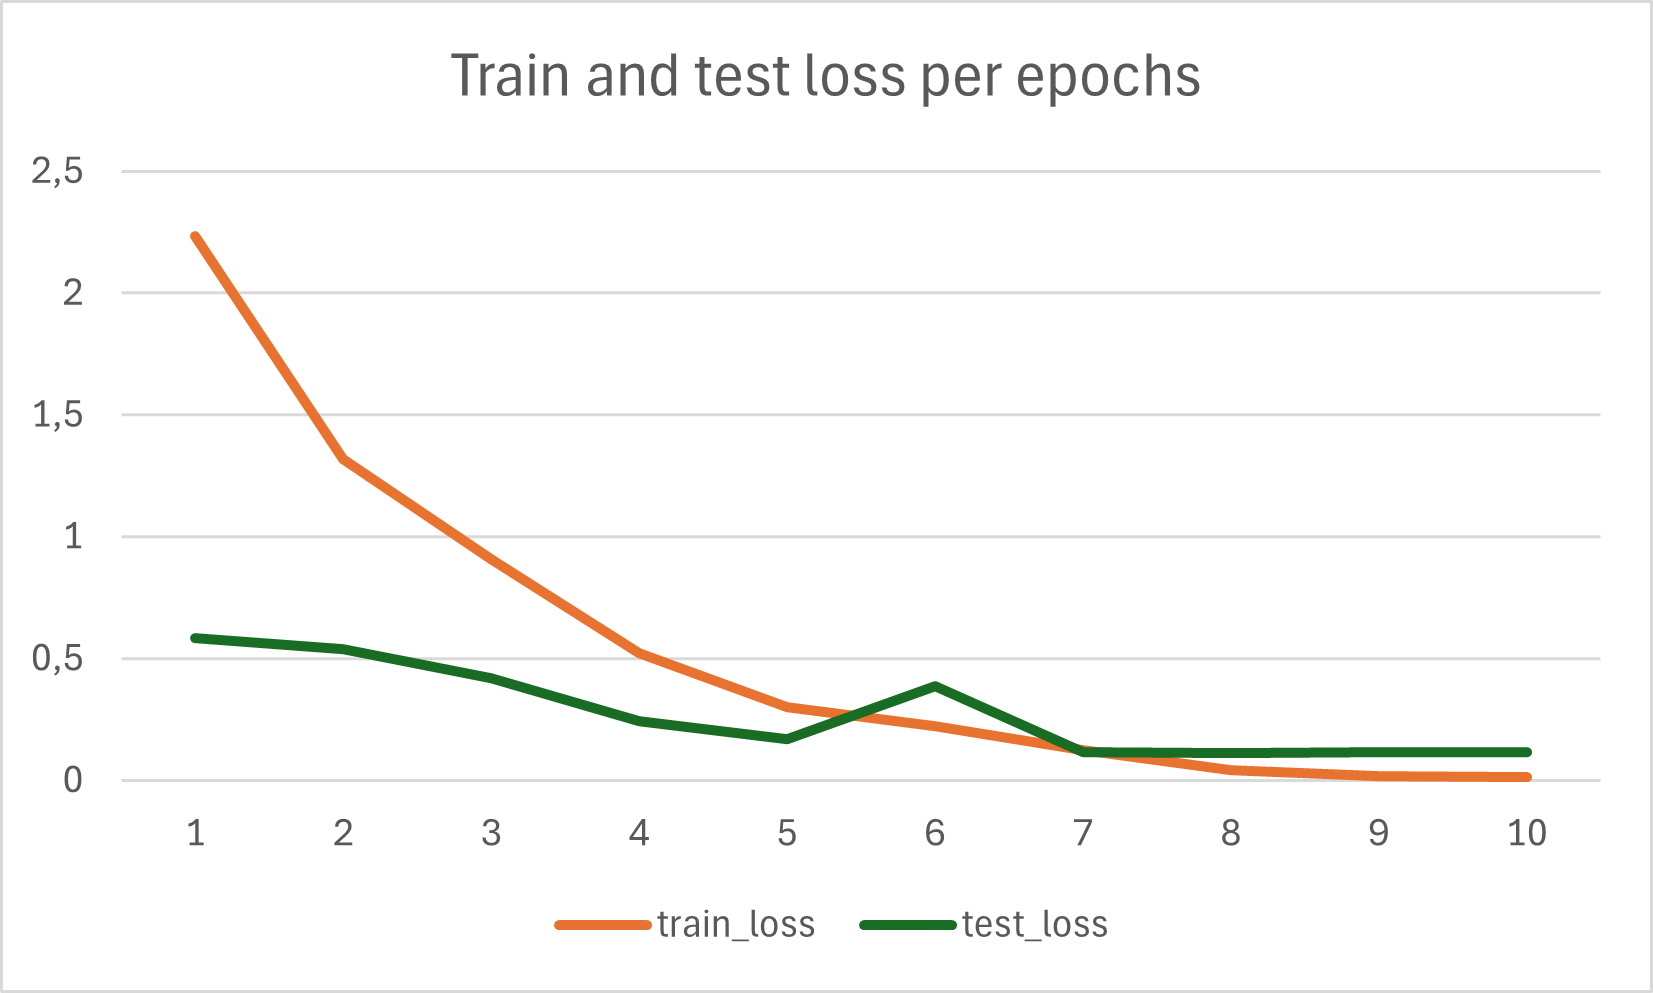
\includegraphics[width=\linewidth]{figures/results/baseline_experiment_loss_per_epoch.png}
\caption{Training and test loss per epoch for the baseline model.}
\label{fig:baseline-loss}
\end{figure}

\vspace{1em}
\begin{figure}[H]
\centering
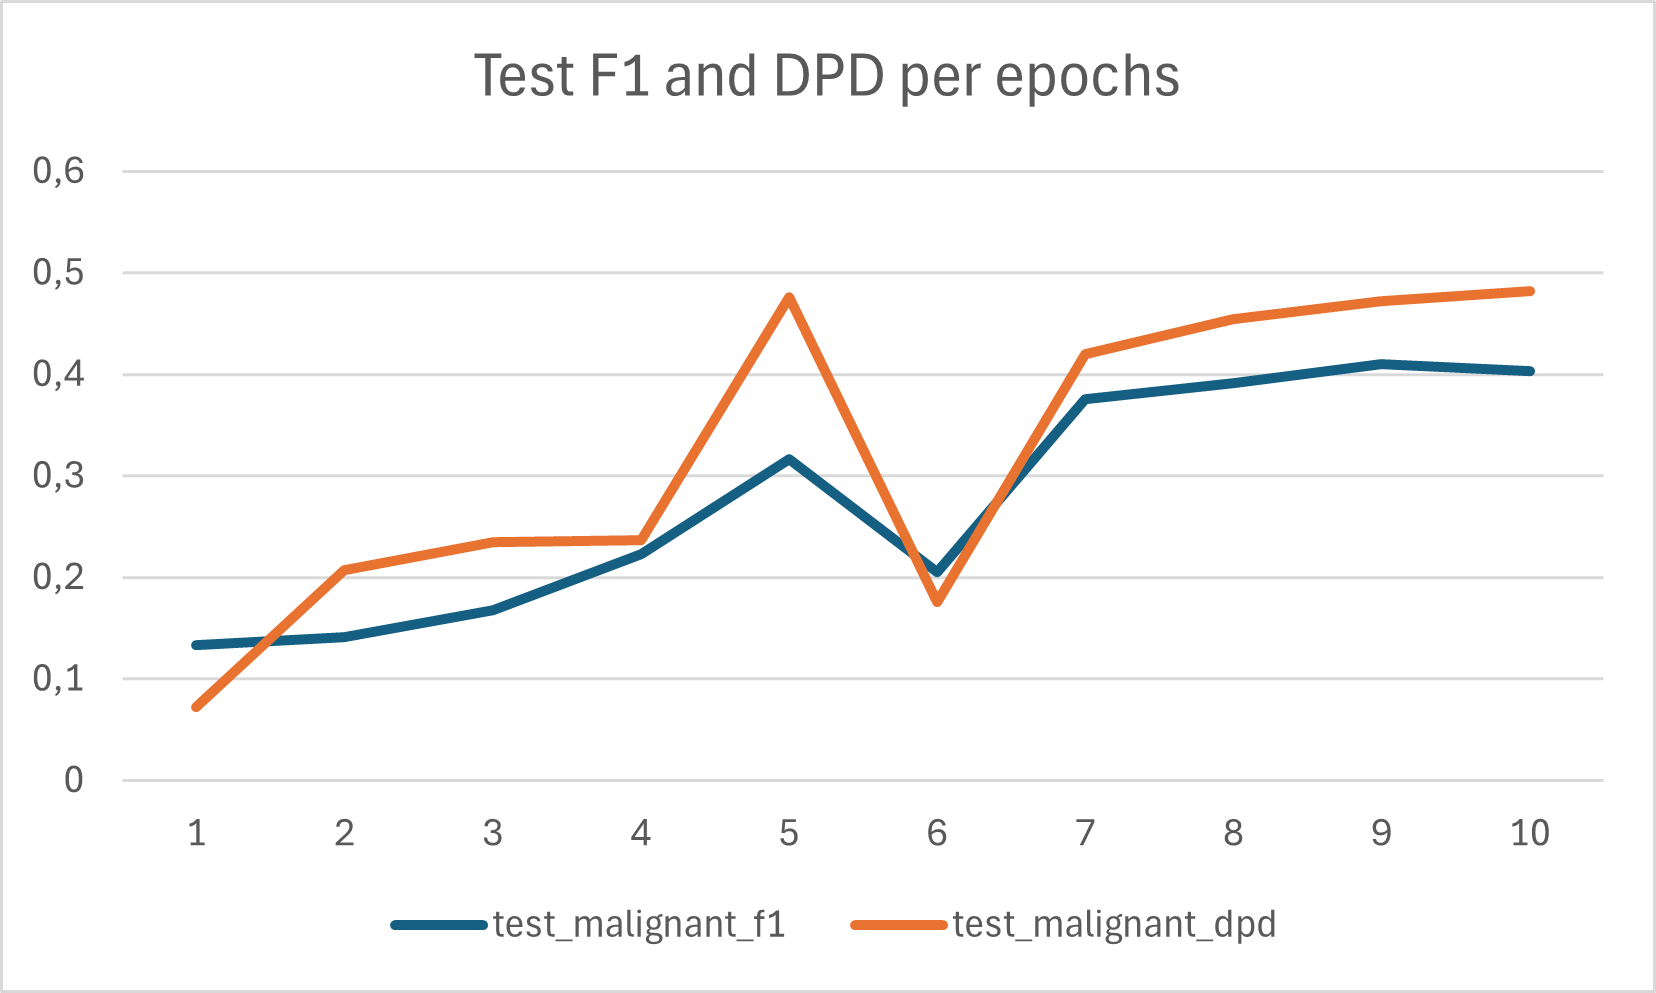
\includegraphics[width=\linewidth]{figures/results/baseline_experiment_metricsper_epoch.png}
\caption{F1 score, recall, and precision of the malignant class across epochs in the baseline model.}
\label{fig:baseline-metrics}
\end{figure}


What we observe in this table and on the graphs is that the model converges on both the training and test sets. Convergence on the training set is evident from the gradual decrease in loss, which approaches zero, and the training accuracy reaching nearly 100\%. This is a common effect we noticed where the model easily learns to find the decision boundary between the smaller number of malignant examples and the more abundant benign ones in the training set, yet this does not translate well to test performance. We also concluded that the test recall from the best epoch, based on the highest F1 score in the 9\textsuperscript{th} epoch (37.22\%), was too low. Our goal then became to improve recall for the malignant class while maintaining the F1 score as much as possible.

\subsection{Baseline vs recall cross entropy}
We immediately started an ablation regarding the performance of recall based loss compared to weighted croos entropy loss. Then we did an ablation of parameter tuning experiments, and here we report the best example. 

\begin{table}[H]
\centering

\caption{Comparison of three configurations showing test accuracy, recall, F1, DPD, and group-wise recall for the malignant class.}
\resizebox{\textwidth}{!}{%
\begin{tabular}{|l|c|c|c|c|c|c|c|c|}
\toprule
\textbf{Experiment} & \textbf{Test Acc} & \textbf{Test Recall} & \textbf{Test F1} & \textbf{Test DPD} & \textbf{Group 0 Recall} & \textbf{Group 1 Recall} & \textbf{Group 3 Recall} & \textbf{Group 4 Recall} \\
\midrule
Baseline CE + IFW & 97.8\% & 37.2\% & 41.0\% & 4.39\% & 76.5\% & 29.3\% & 30.4\% & 43.8\% \\
Recall recall\_based CE & 96.2\% & 50.4\% & 35.8\% & 7.70\% & 76.5\% & 44.8\% & 45.7\% & 56.3\% \\
\bottomrule
\end{tabular}
} % end of resizebox
\label{tab:baseline-vs-variants}
\end{table}

These results show that recall indeed increased, but at the cost of precision, resulting in lower F1 scores. We attempted to scale up the model, but no improvements were observed. Therefore, we decided to take a different approach: we switched to the CIELAB color space. All experiments from this point onward will use CIELAB images.

\subsection{CIELAB colorspace results}

All of the reported results use the same model: ConvNeXt Tiny, adamw optimizer, cosine scheduler, input resolution of 224x224, and CIELAB normalization based on mean and std of ISIC CHallenge datset in CIELAB colorspace.

\begin{table}[H]
\centering
\caption{Comparison of selected ConvNeXt Tiny experiments on CIELAB images.}
\resizebox{\textwidth}{!}{%
\begin{tabular}{|l|c|c|c|c|c|c|c|c|}
\toprule
\textbf{Experiment} & \textbf{Test Acc} & \textbf{Test Recall} & \textbf{Test F1} & \textbf{Test DPD} & \textbf{Group 0 Recall} & \textbf{Group 1 Recall} & \textbf{Group 3 Recall} & \textbf{Group 4 Recall} \\
\midrule
Recall based CE & 93.6\% & 56.2\% & 27.0\% & 12.5\% & 70.6\% & 43.1\% & 63.0\% & 68.8\% \\
OHEM + ifw & 96.6\% & 32.8\% & 28.6\% & 4.91\% & 64.7\% & 22.4\% & 30.4\% & 43.8\% \\
Finetune of 1 for 10 epochs & 91.9\% & 54.7\% & 22.1\% & 18.2\% & 64.7\% & 46.6\% & 58.7\% & 62.5\% \\
Recall based CE 50 epochs & 95.2\% & 43.8\% & 27.4\% & 19.6\% & 82.4\% & 32.8\% & 45.7\% & 37.5\% \\
Oversampler + re & 94.5\% & 49.6\% & 27.5\% & 9.49\% & 82.4\% & 37.9\% & 54.4\% & 43.8\% \\
Focal loss & 97.0\% & 29.9\% & 29.2\% & 4.57\% & 70.6\% & 20.7\% & 30.4\% & 18.8\% \\
\bottomrule
\end{tabular}
} % end of resizebox
\label{tab:selected-experiments}
\end{table}

These experiments showed a slight increase in recall compared to the RGB color space; an improvement of 5.8\%, from 50.4\% to 56.2\%.  
The F1 score consistently remained below the 30\% mark, and we generally observed that higher overall recall was associated with lower DPD values.  
From the table, we can also see that we have not yet reached satisfactory recall levels, as Groups 1 and 3 still show notably lower recall compared to others.
We still haven't taken a look at the fairness of our models, except for DPD, and we will few sections below. We are still aiming to increase the recall.
In the ablation \ref{ap:model_results}, table \ref{tab:oversampler_abl}, we did ablation study concerning which loss to use with oversampler.

\subsection{EfficientNetV2 experiments}
We did and extensive EfficientNetV2 experiment ablation, here we are reporting two of our best runs.

\begin{table}[h!]
\centering
\caption{Performance comparison between EfficientNet-M and Efficient-L models.}
\resizebox{\textwidth}{!}{%
\begin{tabular}{|l|c|c|c|c|c|c|c|c|}
\toprule
\textbf{Experiment} & \textbf{Test Acc} & \textbf{Test Recall} & \textbf{Test F1} & \textbf{Test DPD} & \textbf{Group 0 Recall} & \textbf{Group 1 Recall} & \textbf{Group 3 Recall} & \textbf{Group 4 Recall} \\
\midrule
EfficientNetV2 M + recall based CE + IFW & 92.4\% & 56.9\% & 23.8\% & 14.0\% & 82.4\% & 44.8\% & 58.7\% & 68.8\% \\
EfficientNetV2 L + recall based CE + IFW & 94.0\% & 50.4\% & 26.0\% & 9.65\% & 94.1\% & 39.7\% & 43.5\% & 62.5\% \\
\bottomrule
\end{tabular}
} % end of resizebox
\label{tab:efficient-models}
\end{table}

These models showed little progress in teh direction we wanted: to increase recall and F1 score. EfficientNetV2 M  got the highest recall so far, EfficientNetV2 L struggled with overfitting the train dataset.
We decided to apply heavier transformations: segmentation-aided classification and skin-former based modelling.

\subsection{Segmentation-aided classification and skin-former results}

We aimed to evaluate the performance of the ConvNeXt-Tiny model, which is capable of handling irregular image inputs, on two types of data: segmented images, where only the lesions were visible to the model, and color-transformed images, referred to as the skin-former approach.

\begin{table}[H]
\centering
\caption{Performance of ConvNeXt-Tiny on 224x224 CIELAB images with skin color transformer augmentation and masked skin augmentation.}
\resizebox{\textwidth}{!}{%
\begin{tabular}{|l|c|c|c|c|c|c|c|c|}
\toprule
\textbf{Experiment} & \textbf{Test Acc} & \textbf{Test Recall} & \textbf{Test F1} & \textbf{Test DPD} & \textbf{Group 0 Recall} & \textbf{Group 1 Recall} & \textbf{Group 3 Recall} & \textbf{Group 4 Recall} \\
\midrule
Skin former + Recall based CE & 90.3\% & 66.4\% & 22.3\% & 17.6\% & 88.2\% & 51.7\% & 69.6\% & 87.5\% \\
Skin former + OHEM + IFW & 96.0\% & 31.4\% & 24.8\% & 5.09\% & 58.8\% & 27.6\% & 28.3\% & 25.0\% \\
Masked skin + Recall based CE & 96.0\% & 37.2\% & 25.7\% & 10.1\% & 82.4\% & 24.1\% & 39.1 \% & 31.3\% \\
\bottomrule
\end{tabular}
} % end of resizebox
\label{tab:transformer-results}
\end{table}

The masked skin transformation resulted in a performance decrease compared to previous results. We believe the explanation lies in the fact that we were using pretrained weights on ImageNet, and this data distribution shift proved insurmountable for our model to overcome. 
Additionally, this transformation often produced a higher number of false positives and led to unstable training when not initialized with pretrained weights, as the models easily overfitted the training dataset. We therefore decided not to experiment further with this transformation.
As a result, we turned to the skin-former transformation for ablation studies, aiming to improve these results. It proved easier to train with, yielded a 9.5\% higher recall than EfficientNetV2-M, and produced fewer false positives across demographic groups.
A natural next step was to apply domain-aware training. The following section presents the best of those runs.


\subsection{Domain-aware training}
Here, we report three of our best runs using the skin-former augmentation and domain-aware training setup. We experimented with both domain-independent and domain-discriminative training strategies, and present the results below.


\begin{table}[H]
\centering
\caption{Performance of domain-discriminatively and domain-independently trained ConvNeXt-Tiny models using 224×224 CIELAB images with optional skin-former augmentation.}
\label{tab:domain-transformers}
\resizebox{\textwidth}{!}{%
\begin{tabular}{|l|c|c|c|c|c|c|c|c|}
\toprule
\textbf{Experiment} & \textbf{Test Acc} & \textbf{Test Recall} & \textbf{Test F1} & \textbf{Test DPD} & \textbf{Group 0 Recall} & \textbf{Group 1 Recall} & \textbf{Group 3 Recall} & \textbf{Group 4 Recall} \\
\midrule
Domain discriminative + CE + IFW & 89\% & 72.3\% & 21.5\% & 18.9\% & 88.2\% & 62.1\% & 73.9\% & 87.5\% \\
Domain independent + CE + IFW & 97\% & 19.7\% & 23.5\% & 2.10\% & 29.4\% & 17.2\% & 19.6\% & 18.8\% \\
Domain discriminative + skin former + CE + IFW & 85\% & 23.8\% & 17.4\% & 25.4\% & 82.4\% & 62.1\% & 82.6\% & 87.5\% \\
\bottomrule
\end{tabular}
} % end of resizebox

\end{table}

Domain-independent training underperformed on the test set. It consistently predicted the majority of images as benign, resulting in regularly low recall. Forcing the model to learn the decision boundary between classes only increased the false positive rate and reduced precision. Therefore, we decided not to continue with this training procedure.
On the other hand, the domain-discriminative training procedure yielded the highest recall scores across all runs. The best run increased recall by 8.1\%, reaching a strong overall recall of 74.5\%. When analyzing group-wise recall, the lowest was recorded in Group 1 with 62.1\%, while all other groups achieved well over 80\% recall.

We were willing to sacrifice some precision, which came at the cost of a drop in F1 score, from the baseline of 40\% down to as low as 17.4\%. Given the 49-to-1 imbalance ratio in our dataset, we considered this trade-off acceptable, as we could afford more false positives and a higher false positive rate.

\subsection{Fairness analysis}
We conducted an extensive fairness analysis of most of our models; here, we present a shortened version of the results table. The full table is provided in Appendix~\ref{ap:model_results}.

Our primary condition was that the model must maintain a low false positive rate: our priority was recall, and we could not afford to lower recall in favor of a higher F1 score. This was a general tendency across all models: they would either predict more malignant cases, boosting recall but reducing F1 score due to more false positives, or increase F1 during training at the cost of recall by maintaining a low false positive rate. Some of our experiments, which are discussed in Appendix~\ref{ap:model_results}, either overfitted the training data or, in the case of linear probing with DINOv2, underfitted, resulting in an overwhelming number of false positives, with 100\% recall but precision of only a few percentage points.

It was difficult to establish rigid criteria, but we ultimately used the following thresholds: 
\begin{itemize}
    \item False negative rate over 50\% was considered unacceptable and such models were excluded.
    \item False positive rate over 50\% was another exclusion criterion, which only applied to linear probing experiments (see Appendix~\ref{ap:model_results}).
    \item Recall lower than 50\% was considered insufficient.
    \item Lastly, an F1 score below 20\% was deemed inadequate for inclusion.
\end{itemize}

It is worth noting that only one model per architecture and training configuration was retained. Among models that met these thresholds, the EfficientNetV2-M model achieved 56\% recall and a 24\% F1 score, compared to the best EfficientNetV2-L model, which had a 2\% higher F1 but 6\% lower recall. In this case, we chose the smaller M variant, as higher recall and fewer parameters were prioritized over a marginally better F1 score.
The table summarizing the best-performing models and metrics across the entire validation dataset is presented below:


\begin{table}[H]
\centering
\caption{Comparison of selected experiments across fairness and classification metrics.}
\resizebox{\textwidth}{!}{%
\begin{tabular}{|l|c|c|c|c|c|c|c|c|}
\toprule
\textbf{Experiment} & \textbf{Balanced Acc.} & \textbf{DPD} & \textbf{Eq. Opp.} & \textbf{F1} & \textbf{FNR} & \textbf{FPR} & \textbf{Recall} & \textbf{Selection Rate} \\
\midrule
ConvNeXt-tiny + RGB + recall CE & 73.78\% & 7.70\% & 31.64\% & 35.75\% & 49.64\% & 2.80\% & 50.37\% & 3.79\% \\
ConvNeXt-tiny + CIELAB + recall CE & 75.32\% & 12.50\% & 27.48\% & 26.97\% & 43.80\% & 5.56\% & 56.20\% & 6.61\% \\
ConvNeXt-tiny + skin-former & 78.62\% & 17.55\% & 36.51\% & 22.25\% & 33.58\% & 9.18\% & 66.42\% & 10.38\% \\
ConvNeXt-tiny + domain discriminative train & 80.81\% & 18.86\% & 26.17\% & 21.52\% & 27.74\% & 10.65\% & 72.26\% & 11.93\% \\
EfficientNet-M + recall CE + IFW & 75.04\% & 13.95\% & 37.53\% & 23.82\% & 43.07\% & 6.85\% & 56.93\% & 7.89\% \\
\bottomrule
\end{tabular}
} % end of resizebox
\label{tab:fairness-metrics}
\end{table}

We emphasize that the results discussed here are based on validation over the entire dataset. These metrics offer a broader view of our model performances, but they do not allow for a fine-grained assessment of bias at the individual skin color group level. First, let us examine some general conclusions drawn from this table.

The Demographic Parity Difference (DPD) reaches a maximum of around 19\%, signaling the model with the largest performance disparity across groups. The lowest DPD observed was 8\%. When comparing this with recall, and acknowledging their potential mutual exclusiveness, we see that the model with the highest recall also exhibited the highest DPD, while the model with the lowest recall had the lowest DPD. This could suggest that the best-performing model in terms of recall learned patterns specific to one skin color group more effectively than others. However, this observation alone does not provide a definitive answer as to which model is preferable.

The Equal opportunity metric generally indicated similar performance across models. We stress that this metric was calculated using the validation dataset only and represents the probability of a positive case being correctly identified, conditional on the individual's group. Again, the model with the highest recall showed the lowest equalized opportunity score. However, this metric ranged fairly consistently between 26\% and 37\% across all models.

The model with the highest recall also produced the most predictions, which led to more false positives than other models. This is reflected in its highest false positive rate and highest selection rate. At the same time, it achieved the lowest false negative rate among all models. Naturally, a higher selection rate and false positive rate result in lower precision; thus, it is not surprising that this model also had the lowest F1 score, at 21.52\%.

\subsubsection{Group-level metrics}
Let us further analyze these models of ours. We are now digging deeper: at the per-group prediction level.

\begin{table}[htpb]
\centering
\caption{Per-group performance metrics: ConvNeXt-tiny + RGB + recall CE}
\label{tab:rgb-recallce} 
\begin{tabular}{cccccccc}
\toprule
\textbf{Group} & \textbf{F1} & \textbf{Recall} & \textbf{Accuracy} & \textbf{\begin{tabular}[c]{@{}c@{}}Selection\\ Rate\end{tabular}} & \textbf{\begin{tabular}[c]{@{}c@{}}Balanced \\ Accuracy\end{tabular}} & \textbf{FPR} & \textbf{FNR} \\ \midrule
0              & 60\%        & 76\%            & 94\%              & 9\%                                                               & 86\%                                                                  & 5\%          & 24\%         \\
1              & 31\%        & 45\%            & 97\%              & 3\%                                                               & 71\%                                                                  & 2\%          & 55\%         \\
2              & 31\%        & 46\%            & 94\%              & 5\%                                                               & 71\%                                                                  & 4\%          & 54\%         \\
3              & 46\%        & 56\%            & 91\%              & 10\%                                                              & 75\%                                                                  & 7\%          & 44\%         \\ \bottomrule
\end{tabular}
\end{table}

\begin{table}[htpb]
\centering
\caption{Per-group performance metrics: ConvNeXt-tiny + CIELAB + recall CE}
\label{tab:ciellab-recallce}
\begin{tabular}{cccccccc}
\toprule
\textbf{Group} &
  \textbf{F1} &
  \textbf{Recall} &
  \textbf{Accuracy} &
  \textbf{\begin{tabular}[c]{@{}c@{}}Selection\\ Rate\end{tabular}} &
  \textbf{\begin{tabular}[c]{@{}c@{}}Balanced \\ Accuracy\end{tabular}} &
  \textbf{FPR} &
  \textbf{FNR} \\ \midrule
0 & 62\% & 71\% & 95\% & 8\%  & 83\% & 4\%  & 29\% \\
1 & 21\% & 43\% & 96\% & 4\%  & 70\% & 3\%  & 57\% \\
2 & 24\% & 63\% & 88\% & 12\% & 76\% & 11\% & 37\% \\
3 & 42\% & 69\% & 86\% & 16\% & 78\% & 12\% & 31\% \\ \bottomrule
\end{tabular}
\end{table}

\begin{table}[htpb]
\centering
\caption{Per-group performance metrics: ConvNeXt-tiny + skin-former}
\label{tab:skin-former}
\begin{tabular}{cccccccc}
\toprule
\textbf{Group} &
  \textbf{F1} &
  \textbf{Recall} &
  \textbf{Accuracy} &
  \textbf{\begin{tabular}[c]{@{}c@{}}Selection\\ Rate\end{tabular}} &
  \textbf{\begin{tabular}[c]{@{}c@{}}Balanced \\ Accuracy\end{tabular}} &
  \textbf{FPR} &
  \textbf{FNR} \\ \midrule
0 & 59\% & 88\% & 93\% & 12\% & 91\% & 7\%  & 12\% \\
1 & 16\% & 52\% & 93\% & 7\%  & 73\% & 6\%  & 48\% \\
2 & 19\% & 70\% & 83\% & 18\% & 77\% & 16\% & 30\% \\
3 & 39\% & 88\% & 81\% & 24\% & 84\% & 20\% & 13\% \\ \bottomrule
\end{tabular}
\end{table}

\begin{table}[htpb]
\centering
\caption{Per-group performance metrics: ConvNeXt-tiny + domain discriminative}
\label{tab:domain-discriminative}
\begin{tabular}{cccccccc}
\toprule
\textbf{Group} &
  \textbf{F1} &
  \textbf{Recall} &
  \textbf{Accuracy} &
  \textbf{\begin{tabular}[c]{@{}c@{}}Selection\\ Rate\end{tabular}} &
  \textbf{\begin{tabular}[c]{@{}c@{}}Balanced \\ Accuracy\end{tabular}} &
  \textbf{FPR} &
  \textbf{FNR} \\ \midrule
0 & 56\% & 88\% & 92\% & 13\% & 90\% & 8\%  & 12\% \\
1 & 17\% & 62\% & 92\% & 8\%  & 77\% & 8\%  & 38\% \\
2 & 19\% & 74\% & 82\% & 20\% & 78\% & 18\% & 26\% \\
3 & 36\% & 88\% & 78\% & 27\% & 83\% & 22\% & 13\% \\ \bottomrule
\end{tabular}
\end{table}

\begin{table}[htpb]
\centering
\caption{Per-group performance metrics: EfficientNet-M}
\label{tab:efficientnet-m}
\begin{tabular}{cccccccc}
\toprule
\textbf{Group} &
  \textbf{F1} &
  \textbf{Recall} &
  \textbf{Accuracy} &
  \textbf{\begin{tabular}[c]{@{}c@{}}Selection\\ Rate\end{tabular}} &
  \textbf{\begin{tabular}[c]{@{}c@{}}Balanced \\ Accuracy\end{tabular}} &
  \textbf{FPR} &
  \textbf{FNR} \\ \midrule
0 & 55\% & 82\% & 92\% & 12\% & 87\% & 7\%  & 18\% \\
1 & 18\% & 45\% & 95\% & 5\%  & 70\% & 5\%  & 55\% \\
2 & 21\% & 59\% & 87\% & 13\% & 73\% & 12\% & 41\% \\
3 & 37\% & 69\% & 84\% & 19\% & 77\% & 15\% & 31\% \\ \bottomrule
\end{tabular}
\end{table}

This is a substantial amount of data to process. So, what are we aiming to do? In Section~\ref{subsec:statistical_fairness}, we aim to assess the fairness of our models at the image level. While we have already evaluated fairness at the dataset level, we now focus on ensuring that our models are fair across individual skin color groups.

Group 0 represents individuals with the lightest skin tone, while Group 4 represents those with the darkest. In each table, we show the sample count per group and various evaluation metrics.

Our priorities are: (1) high recall (i.e., low false negative rate), and (2) minimal recall disparity across skin tone groups.

In Table~\ref{tab:rgb-recallce}, we observe that Groups 1 and 2 have recalls of only 45\% and 46\%, respectively, corresponding to false negative rates (FNRs) of 55\% and 54\%. A similar pattern appears in Table~\ref{tab:ciellab-recallce}, where the recall for the most frequent group is just 43\%. Table~\ref{tab:efficientnet-m} also shows modest recall in these groups, around 45\%.

Model~\ref{tab:rgb-recallce} was discarded due to low recall in the most common groups and high false negative errors. Although Model~\ref{tab:ciellab-recallce} had even higher false negative errors and lower recall in the highest-performing group, it too was excluded. EfficientNet-M (Table~\ref{tab:efficientnet-m}) showed slightly lower recall overall but had smaller false negative errors, with the highest error observed only in the darkest skin group. We decided to proceed with it. The deciding factor was the difference in recall across groups: ConvNeXt-tiny (RGB) had a recall disparity of 31\%, ConvNeXt-tiny (CIELAB) had 28\%, while EfficientNet-M had the lowest at just 14\%, even better than the skin-former variant at 18\%.

Among the remaining models in Tables~\ref{tab:skin-former},~\ref{tab:domain-discriminative}, and~\ref{tab:efficientnet-m}, F1 scores across groups are nearly identical. All models exhibit slight selection rate bias toward underrepresented groups. The domain-discriminatively trained ConvNeXt-tiny model stands out with the highest recall across all groups, with the lowest recall still at a respectable 62\%. The skin-former augmented variant of ConvNeXt-tiny also performed well in terms of recall.

Overall, the domain-discriminative ConvNeXt-tiny model appears to be the most fair and best performing in terms of group-wise recall. Given its strong recall and the lowest in-between group recall disparity, it emerges as our top candidate. The only mild concern is the variation in selection rate across groups, as reflected by the false positive rate (FPR). However, this is not particularly alarming for our use case (detecting malignant lesions), since we prioritize reducing false negatives. In this context, a higher FPR is acceptable, especially when it helps avoid missing malignant cases.

So far, the best-performing model is the domain-discriminatively trained ConvNeXt-tiny. We finalize this analysis in Section~\ref{subsec:statistical_fairness}.



\subsection{Statistical fairness estimation}
\label{subsec:statistical_fairness}

Previous discussions and results only considered group-level and disparity metrics as means to measure and quantify fairness. With the following experiments, we want to go a step further and look at the fairness of our models from a different point of view and analyse their performance at the image level. Because we are doing classification, we will be using the predicted posterior probabilities of the malignant class $P(y=\text{malignant} \mid x)$ as image-level performance metrics. By doing this, the fairness we are testing for becomes equal confidence across skin color groups. This section will focus on three models listed in table \ref{tab:anova_experiments} that have shown the best overall performance and fairness.  

\begin{table}[htpb]
\centering
\caption{Best-performing experiments selected for further fairness analysis.}
\label{tab:anova_experiments}

\begin{tabular}{ll}
\toprule
\textbf{Alias} & \textbf{Experiment} \\ \midrule
Experiment 1   &  ConvNeXt-tiny + skin-former  \\
Experiment 2   &  ConvNeXt-tiny + domain discriminative \\
Experiment 3   &  EfficientNet-M  \\ \bottomrule
\end{tabular}
\end{table}

\subsubsection{Ground-truth positive subset}

We want to test whether trained models behave differently across skin color groups on ground-truth malignant samples, regardless of whether or not they were correctly labelled by the model. This gives us an overall view of the fairness of each model and checks for confidence disparities in all malignant samples. Table \ref{tab:anova_gt} compares our three best-performing models and shows the mean posterior probabilities for each skin color group and corresponding one-way ANOVA statistics. The primary and alternative hypotheses for this experiment are:

\begin{center}
\begin{tabular}{rl}
    $H_0 \quad\hdots\quad$  & Mean probabilities $P(y=\text{malignant} \mid x)$ are equal for GT \\
                            & malignant samples across all skin color groups \vspace{0.3em} \\
    $H_1\quad\hdots\quad$   & At least one mean probability is different from the rest
\end{tabular}
\end{center}

\begin{table}[htpb]
\centering
\caption{Mean malignant-class posterior probabilities of ground-truth positive samples for different skin tone groups. Three different models are compared using the shown one-way ANOVA statistics and p-values.}
\label{tab:anova_gt}

\begin{tabular}{cccc}
\toprule
\multicolumn{1}{c}{\textbf{\begin{tabular}[l]{@{}c@{}}Skin tone\\ group\end{tabular}}} & \textbf{Experiment 1} & \textbf{Experiment 2} & \textbf{Experiment 3} \\ \midrule
0                                                                                      & $0.838 \pm 0.323$     & $0.320 \pm 0.280$     & $0.784 \pm 0.334$     \\
1                                                                                      & $0.508 \pm 0.410$     & $0.230 \pm 0.272$     & $0.435 \pm 0.410$     \\
2                                                                                      & $0.658 \pm 0.376$     & $0.251 \pm 0.253$     & $0.581 \pm 0.404$     \\
3                                                                                      & $0.735 \pm 0.285$     & $0.261 \pm 0.223$     & $0.653 \pm 0.361$    \vspace{0.3em}\\ 
\multirow{2}{*}{ANOVA}                                                                 & $F = 4.142$           & $F = 0.520$           & $F = 3.983$           \\
                                                                                       & $p = 0.008$           & $p = 0.669$           & $p = 0.009$           \\ \bottomrule
\end{tabular}
\end{table}

The ANOVA results show that we can discard $H_0$ with a $0.05$ level of significance in experiments 1 and 3. This indicates the presence of skin-color bias in those two models; more specifically that those models are not equally confident in their decisions across groups. Looking at the mean values per group, models 1 and 3 seem to give more opportunities (higher confidence) to the minority skin groups. However, knowing that group 1 had the majority in the training data, we can safely assume that the results on other groups are overly optimistic. The mean values for experiment 2 suggest a very stable confidence across skin color groups, despite the fact that the training dataset was highly imbalanced. Because this analysis includes samples that were mislabelled as benign, all three models have a high variance.



\subsubsection{True positive subset}

Looking only at the samples that were correctly labelled as malignant, we can check if our model was less confident to assign that label to samples from different skin color groups. The results of the following statistical test are shown in table \ref{tab:anova_tp}.

\begin{center}
\begin{tabular}{rl}
$H_0 \quad\hdots\quad$  & Mean probabilities $P(y=\text{malignant} \mid x)$ are equal for \\
                        & correctly classified samples across all skin color groups \vspace{0.3em} \\
$H_1\quad\hdots\quad$   & At least one mean probability is different from the rest \\
\end{tabular}
\end{center}

\begin{table}[htpb]
\centering
\caption{Mean malignant-class posterior probabilities of samples correctly classified as malignant for different skin tone groups. Three different models are compared using the shown one-way ANOVA statistics and p-values.}
\label{tab:anova_tp}

\begin{tabular}{cccc}
\toprule
\textbf{\begin{tabular}[c]{@{}c@{}}Skin tone\\ group\end{tabular}} & \textbf{Experiment 1} & \textbf{Experiment 2} & \textbf{Experiment 3} \\ \midrule
0                                                                  & $0.950 \pm 0.112$     & $0.650 \pm 0.049$     & $0.930 \pm 0.120$     \\
1                                                                  & $0.879 \pm 0.158$     & $0.639 \pm 0.047$     & $0.865 \pm 0.157$     \\
2                                                                  & $0.885 \pm 0.148$     & $0.639 \pm 0.048$     & $0.903 \pm 0.118$     \\
3                                                                  & $0.827 \pm 0.157$     & $0.627 \pm 0.069$     & $0.881 \pm 0.134$    \vspace{0.3em}\\
\multirow{2}{*}{ANOVA}                                             & $F = 1.612$           & $F = 0.131$           & $F = 0.741$           \\
                                                                   & $p = 0.192$           & $p = 0.941$           & $p = 0.531$           \\ \bottomrule
\end{tabular}
\end{table}

When only considering true positive predictions, we see no statistically significant evidence of confidence disparities and we fail to reject the null hypothesis in all three experiments. Unlike the results of the previous ANOVA analysis, this analysis did not reveal any biases in experiments 1 and 3. This further shows that, looking only at true positive samples, we get a slightly biased and less general view of our model's fairness. Thus, we suspect that the models in experiments 1 and 3 could be fair (consistently confident) in the cases that they are correct, but they do in general show some bias. As was expected and previously noted, the variances in probability are drastically lower than in table \ref{tab:anova_gt}.


\section{Final Model}

Throughout Section~\ref{sec:results}, we aimed to tell the story of how we developed and refined our models. We conducted numerous experiments, tests, and applied various techniques to optimize performance while focusing rigorously on model fairness. 

After the final analysis in Subsection~\ref{subsec:statistical_fairness}, we conclude that the best-performing model is the ConvNeXt-Tiny, trained on 224x224 CIELAB images using domain-discriminative training for 10 epochs. The model was optimized using the standard cross-entropy loss, weighted by inverse frequency weighting. This model achieves a recall of 72.3\%, a mean per-group recall ($mR$) of 78\%, an F1 score of 21.5\%, a balanced accuracy of 80.81\%, a demographic parity difference (DPD) of 18.8\%, and a false positive rate (FPR) of 10.65\%. Statistical testing revealed no indication of group-level bias at the image level. All metrics, both on the overall validation set and across individual skin color groups, suggest that the model performs fairly and consistently. Therefore, this is the model we are submitting as our final solution. Its configuration will be made publicly available, and its checkpoint will be served during inference.
